\documentclass[a4paper]{report}


\usepackage[a4paper,width=150mm,top=25mm,bottom=25mm]{geometry}
\usepackage{amsmath}
\usepackage{multicol}
\usepackage{caption}
\usepackage{subcaption}
\usepackage{graphicx}
\usepackage{amssymb}
\usepackage{comment}
\usepackage[utf8]{inputenc}
\usepackage{booktabs} % tabelle belle che fa Eugenia!
\usepackage{xcolor}
\usepackage{etoolbox}
\usepackage{siunitx} % per fare numeri e unità di misura belle

\usepackage[backend=biber,style=numeric,sorting=none]{biblatex}%style=alphabetic 
\addbibresource{bib/bibliography.bib}

\renewcommand*\contentsname{Summary}

\newcommand{\red}[1]{\textcolor{red}{#1}}
\begin{document}

\tableofcontents



\chapter{Introduction}
Since the 1980s, when the fabrication of device with very small electrodes (50-100 \si{\um}) became a practical possibility, pixel detectors have been widely employed for imaging and tracking charged particles in the vertex region of experiments at accelerators. Thanks to their excellent spatial resolution, today even better than \SI{10}{\um}, they allow for true three dimensional space-point determination even at high particle fluxes and in particular for the identification of secondary vertices of short-lived particles such as $\tau$ and B mesons.
Requirement imposed by accelerators are stringent and they will become even more so with the increase of luminosity; in this scenario CMOS Monolithic Active Pixel Sensors (MAPS), based on the technology of CMOS cameras, are being developed to improve the performance of the hybrid pixel detectors, which currently constitute the state-of-art for large scale pixel detector, in particular by reducing the amount of material, power consumption and pixel dimension. Indeed, while hybrid pixels are made by two parts, the sensor and the electronics, welded together through microconnections, the MAPS integrate them all on the same wafer.

Experiments such as ALICE at LHC and STAR at RHIC have already introduced the CMOS MAPS technology in their detectors. ALICE Tracking System (ITS2), upgraded during the LHC long shut down in 2019-20, was the first large-area ($\sim$10 \si{m^2}) silicon vertex detector based on CMOS MAPS. Thanks to the reduction of the material budget, ITS2, which uses the ALPIDE chip developed by ALICE collaboration, obtained an amazing improvement both in the position measurement and in the momentum resolution, improving the efficiency of track reconstruction for particle with very low transverse momentum (by a factor 6 at $p_{T}\sim$ 0.1 \si{GeV/c}).
Further advancements in CMOS MAPS technology are being aggressively pursued for the ALICE ITS3 and the Belle II vertex detector upgrades (both foreseen around 2026-27), and by the R$\&$D53 collaboration for the upgrade at HL-LHC, with the goals of further reducing the sensor thickness and improving the readout speed of the devices, while keeping power consumption at a minimum.

Beside tracking, the development of pixel detectors is a very active field with many applications: a noteworthy example of detector originally used in particle physics and later employed for medical imaging, in space detectors and for art authentication, is Medipix, a hybrid system developed at CERN within the Medipix collaboration.
Among medical applications, a possible use of CMOS MAPS could be in dosimetry: in the last few years the search of radiotherapy oncological treatments with high intensity beams (FLASH mode) is requiring new dosimeters, both for the therapies as well as new beam-monitors (especially for focused very high energy electron beams), which are capable of deal with extreme dose rate (up to 40 \si{Gy/s}).

I have studied the characteristics of two ALPIDE-like CMOS MAPS chips and tested them under different front end configuration. The first chip, the TJ-Monopix1 from the Monopix series, is a TowerJazz MAPS fabricated in 180 nm CMOS technology with an active area of 1$\times$2~\si{cm\squared} (448$\times$224 pixels) and is one of the prototypes for the Belle II vertex detector upgrade. The second chip, called Main Demonstrator-1, has an active area of 1.28$\times$1.28~\si{cm\squared} (512$\times$512 pixels) is produced by LFoundry in 110 nm CMOS technology and designed by the ARCADIA (Advanced Readout CMOS Architectures with Depleted Integrated sensor Arrays) group; it is intended to be a general purpose device with possible use in medical scanners, space experiments, future lepton colliders and also possibly X-ray applications with thick substrates.  
The main differences between the two chips are in the output signal type and in the readout sequence of the matrix. Concerning the former, TJ-Monopix1 returns an analog output information, that is the time over threshold of the pulse, which can be related with the charge released by the particle in the sensor, while MD1 returns only a digital information; regarding the latter, instead, TJ-Monopix1 has a completely sequential readout, while MD1 roughly combines the information of the hits before the readout in order to reduce the data transmission time.

I have set up the test systems for the two chips in the INFN clean laboratories and characterized the devices electrically and with radioactive sources in terms of threshold, noise, dead time and analog response.
The mean minimum stable threshold evolved through different generation of chips and nowadays it is less than \SI{500}{e-}, allowing thinner sensors with smaller signals: TJ-Monopix1 has proven to be in agreement with this trend, having a threshold of $\sim$\SI{400}{e-}, to be compared with the \SI{2000}{e-} signal expected for a minimum ionizing particle in an epitaxial layer of \SI{25}{\um}. 
Moreover, since one of the main challenges of MAPS are the differences between pixels due to process parameters variation across the wafer, which make the sensor response nonuniform, I have measured the threshold and noise dispersion across the matrix, which I found to be \SI{40}{e-} and \SI{2}{e-} respectively.
I have also studied the response of the analog signal recorded by TJ-Monopix1, that is the time over threshold, and performed a calibration of its absolute value using a Fe55 X-ray source.
All these measurements are important to verify the design parameters of the chip and to validate the chip simulation. 

As conclusion of the measurement campaign, we have tested TJ-Monopix1 at very high intensity using the electron beam of the new ElectronFlash accelerator designed for both medical research and R$\&$D in FLASH-radiotherapy and recently installed at Santa Chiara hospital in Pisa. I have participated in the design of the setup needed for testbeam measurement and I am currently working on the analysis of the data collected. 

\chapter{Pixel detectors}
\input{tex/Chip}

\chapter{Use of pixels detector}
There always was a tight relation between the development of cameras and pixel detectors since 1969, when the idea of CCDs, thanks to whom Boyle and Smith were awarded the Nobel Prize in Physics in 2009, revolutionized photography allowing light to be captured electronically instead of on film. 
Even though the CMOS technology was already known when CCDs spread, the costs of productions were too high to allow the diffusion of these sensors for which needed to wait untill 1990s. From that period on, the fast diffusion of CMOS was mainly due to the less cost than CCD, and the less power required for supply. 

The principal use cases of pixel detectors are particle tracking and imaging: in the former case individual charged particles have to be identified, in the latter instead an image is obtained by the usually un-triggered accumulation of the impinging radiation. 
Also the demands on detectors performance depends on their usage, in particular tracking requires high spatial resolution, fast readout and radiation hardness. 

For scientific imaging, instead, the applications vary from atrophysics and medical imaging to studies of protein dynamics, \red{altro?} and art authentication, for example. 
The counting mode represents the principal imaging tecnique, a direct 

\section{Tracking in HEP}
    Historically, the first pixel detector employed in particle physics was a CCD: it was installed in the spectrometer at the CERN’s Super Proton Synchrotron (SPS) by the ACCMOR Collaboration (Amsterdam, CERN, Cracow, Munich, Oxford, RAL) at mid 1980s, with the pourpose of studing the recently-discovered charm particles.
    The second famous usage of CCDs took place at SLAC in the Large Detector (SLD) during the two years 1996-98. From that period on particle tracking in experiments have been transformed radically: it was mandatory for HEP experiments to build a inner vertex detector. 
    In 1991, the more demanding environments led to the development of hybrid pixel detectors: a dedicated collaboration, RD19, was established at CERN with the specific goal to define a semiconductor micropattern detector with an incorporated signal processing at a microscopic level. 
    In those years a wide set of prototypes of hybrid pixel has been manufactured; among the greatest productions a mention goes to the ATLAS and CMS vertex detector, \red{..}.
    Infact, from the middle of 2013 a second collaboration, RD 53, has been established with the new goal to find a pixel detector suitable for phase II future upgrades of those experiments. Even if the collaboration is specifically focused on design of hybrid pixel readout chips, also monolithic options have been taken in account for their advantageous charateristics. Requirements imposed by HL-LHC will become tigher in time: for example, a dose and radiation of \SI{5}{Mrad} and \si{10 {16}}{NIEL} are exepcted after 5 years of operation. Time resolution, material budget and power consumption are also issues for the upgrade: a time resolution better than \SI{25}{ns} for a bunch crossing frequency of \SI{40}{MHz}, a material budget lower than 2\% and a power consuption lower than  \SI{500}{mW/cm\squared} are required. 

    Amidst the solutions proposed 3D silicon detector, invented by Sherwood Parker in 1995, and MAPS are the most promising. In 3D sensors the electrode is a narrow column of n-type implanted vertically across the bulk instead of being implanted on the wafer's surface. 
    The charge produced by the impinging particle is then drifted transversally within the pixel, and, as the mean path between two electrode can be soufficent low, the trap probability is not an issue. 
    3D pixels have been already proved in ATLAS, for the insertable B layer (IBL),\red{qualcosa? tipo anno e rif a caso.}
    Even if 3D detector are adequately radiation hard, MAPS architecture looked very promising from the beginning: they overcome both the CCDs long reading time and the hybrid problems (I have already explained in section \ref{sec:} the benefits of MAPS). 
    Experiments such as ALICE at LHC and STAR at RHIC have already introduced the CMOS MAPS technology in their detectors. ALICE Tracking System (ITS2), upgraded during the LHC long shut down in 2019-20, was the first large-area ($\sim$10 \si{m\squared} ) silicon vertex detector based on CMOS MAPS.
    \red{ECCO UN MOTIVO 'FISICO' PER CUI SI GUARDA AI MAPS CHE CONTESUALIZZA LA NECESSITÀ DI BASSO SPESSORE: Excess material in the forward region of tracking systems such as time-projection and drift chambers, with their heavy endplate structures, has in the past led to poor track reconstruction efficiency, loss of tracks due to secondary interactions, and excess photon conversions. In colliders at the energy frontier (whether pp or e+e-), however, interesting events for physics are often multi-jet, so there are nearly always one or more jets in the forward region.\\}
    \subsection{Hybrid pixels at LHC: ATLAS, CMS and LHC-b}
        \textbf{ATLAS}\\
        Com'è fatto il rivelatore e vari test per upgrade\\
        Monopix, 3D sensor\\\\
        \textbf{CMS}\\\\
        \textbf{LHC-b} \\
        The latest experiment to upgrade from strips to pixels is LHCb, which has an impressive track record of b and charm physics. Its adventurous Vertex Locator (VELO).
        he latest experiment to upgrade from strips to pixels is LHCb, which has an impressive track record of b and charm physics. Its adventurous Vertex Locator (VELO)
        \\\\


    \subsection{A DEPFET example: Belle-II}
        

    \subsection{CMOS MAPS: ALICE and STAR}
        \textbf{ALICE}\\
        ALICE (A Large Ion Collider Experiment) is a detector dedicated to heavy-ion physics and to the study of the condensed phase of the chromodynamics at the LHC.
        The tracking detector consists of the Inner Tracking System (ITS), the gaseous Time Projection Chamber (TPC) and the Transition Radiation Detector (TRD) and those are embedded in a magnetic field of \SI{0.5}{T}. The ITS is made by six layers of detectors, two for each type, from the interaction point outwards: Silicon Pixel Detector (SPD), Silicon Drift Detector (SDD) and Silicon Strip Detector (SSD).         
        Contrary to the others LHC experiments, ALICE tracker in placed in a quite different environments: the expected dose is smaller by two order of magnitude and the rate of interactions is few \si{MHz} instead of \SI{40}{MHz}, but the number of particles comes out of each interaction is higher (the SPS is invested by a density of particles of $\sim$\SI{100}{1/cm\squared}).  
        The reconstruction of very complicated events whit a large number of particle is a challenge, hence to segment and to minimize the amount of material, which may cause secondary interaction complicating futher the event topology, is considered a viable strategy. 
        
        \red{Upgrade con Monopix1}
        Thanks to the reduction of the material budget, ITS2, which uses the ALPIDE chip developed by ALICE collaboration, obtained an amazing improvement both in the position measurement and in the momentum resolution, improving the efficiency pf track reconstruction for particle with very low transverse momentum (by a factor 6 at pT $\sim$ 0.1 GeV/c). Further advancements in CMOS MAPS technology are being aggressively pursued for the ALICE ITS3 vertex detector upgrades (foreseen around 2026-27), with the goals of further reducing the sensor thickness and improving the readout speed of the devices, while keeping power consumption at a minimum.\\\\
        \textbf{STAR}\\
        MIMOSA-28 devices for the first MAPS-based vertex detector: a 356 Mpixel two-layer barrel system for the STAR experiment at Brookhaven’s Relativistic Heavy Ion Collide

\section{Application in medical imaging}
    \subsection{Medipix and Timepix}
    A noteworthy example of detector originally used in particle physics, and later employed mainly for medical imaging, but also in space and for art authentication, is Medipix, a hybrid system developed at CERN within the Medipix collaboration usato anche da LHC-b (Timepix).\\
    \subsection{Applicability to FLASH radiotherapy}

\chapter{TJ-Monopix1}
TJ-Monopix1 is a small electrode DMAPS with fast R/O capability, fabricated by TowerJazz foundry in 180 nm CMOS imaging process.
It is part, together with prototypes from other series such as TJ-MALTA, of the ongoing R$\&$D efforts aimed at developing DMAPS in commercial CMOS processes, that could cope with the requirements at accelerator experiments.
Both TJ-Monopix and TJ-MALTA series \cite{MALTA}, produced with the same technology by TowerJazz (the timeline of the foundry products is shown in figure \ref{fig:TJ180nm}), are small electrode demonstrators and principally differ in the readout design: while Monopix implements a column-drain R/O, an asynchronous R/O without any distribution of BCID has been used by TJ-Malta in order to reduce power consumption.

\begin{figure}[h!]
    \centering
    \includegraphics[width=.95\linewidth]{figures/Monopix1/TJ180nm.png}
    \caption{Timeline in TowerJazz productions in 180 nm CMOS imaging process}
    \label{fig:TJ180nm}
\end{figure} 

Another Monopix series, but in 150 nm CMOS technology, has been produced by LFoundry~\cite{LF-Monopix}.
The main differences between the LF-Monopix1 and the TJ-Monopix1 (summarized in table \ref{tab:LF-TJ-Monopix}), lay in the sensor rather than in the readout architecture, as both chips implements a fast column drain R/O with ToT capability \cite{LF-TJ-Monopix-short}\cite{LF-TJ-Monopix-long}.
Concerning the sensors, either are based on a p-type substrate, but with slightly different resistivities; in addition LFoundry pixels are larger, thicker and have a large fill factor (the very deep n-well covers $\sim$55$\%$ of the pixel area). The primary consequence is that LF-Monopix1 pixels have a higher capacity resulting in higher consumption and noise. As I discussed in section \ref{sec:small-large-fill-factor},  the fact that LF-Monopix has a large fill factor electrode is expected to improve its radiation hardness. Indeed, a comparison of the perfomance of the two chips showed that TJ-Monopix suffers a comparatively larger degradation of efficiency after irradiation, due to the low electric field in the pixel corner; on the other hand, a drawback of the large fill factor in LF-Monopix is a significant cross-talk.
\begin{table}
    \begin{center}
    \begin{tabular}{|c | c |c |}
    \hline
    & LF-Monopix1 & TJ-Monopix1\\
    \hline
    \hline
    Resistivity & $>$\SI{2}{k\Omega cm}& $>$\SI{1}{k\Omega cm}\\
    Pixel size & 50  $\times$ 250\si{\um\squared} & 36  $\times$ 40 \si{\um\squared} \\
    Depth & 100-750 \si{\um} & \SI{25}{\um} \\
    Capacity & $\sim$ \SI{400}{fF} & $\sim$ \SI{3}{fF}\\
    Preamplifier & charge & voltage \\
    Threshold trimming & on pixel (4-bit DAC) & global threshold\\
    ToT & 8 bits & 6 bits\\
    Consumption & $\sim$  300\si{mW/cm\squared}& $\sim$  120\si{mW/cm\squared} \\
    Threshold & 1500 $e^-$ & $\sim$ 270 $e^-$ \\
    ENC & 100 $e^-$ & $\sim$ 30 $e^-$\\
    \hline
    \end{tabular}
    \caption{Main characteristics of Monopix1 produced by TowerJazz and LFoundry \cite{LF-TJ-Monopix-short}\cite{LF-TJ-Monopix-long}}
    \label{tab:LF-TJ-Monopix}
    \end{center}
 \end{table}

The TJ-Monopix1 chip contains, apart from the pixels matrix, all the required support blocks used for configuration and testing: 
\begin{itemize}
    \item  the whole matrix contains 224 $\times$ 448 pixels, yielding a total active area approximately equal to \SI{145}{mm\squared} over a total area of 1$\times$2\si{cm\squared};
    \item at the chip periphery are placed some 7-bit Digital to Analog Converter (DAC), used to generate the analog bias voltage and current levels and to confiugure the FE; 
    \item at the EoC is placed a serializer to transferred datas immediately, indeed no trigger memory is implemented in this prototypes;
    \item the matrix power pads are distributed at the sides
    \item four pixels which have analog output and which can be monitored with an oscilloscope, and therefore used for testing
\end{itemize}    
Pixels are grouped in 2$\times$2 cores (fig. \ref{fig:pixels_core}): this layout allows to separate the analog and the digital electronics area in order to reduce the possibile interference between the two parts. In addition it semplifies the routing of data as pixels on double column share the same column-bus to EoC. Therefore pixels can be addressed through the physical column/row or through the logical column/row, as shown in fig. \ref{fig:column_order}: in figure is also highlighted the token propagaion path, whose I will discuss later.

\begin{figure}[h!]
    \begin{subfigure}{.5\textwidth}
    \centering
    \includegraphics[width=.98\linewidth]{figures/Monopix1/Monopix1_2x2pixelsgroup.png}
    \caption{Layout of a core containing 4 pixels. The analog FE and the digital part are separated in order to reduce cross-talk be}
    \label{fig:pixels_core}
    \end{subfigure}
    \begin{subfigure}{.5\textwidth}
    \centering
    \includegraphics[width=.88\linewidth]{figures/Monopix1/column_order.png}
    \caption{}
    \label{fig:column_order}
    \end{subfigure}
\end{figure}

\begin{table}
    \begin{center}
    \begin{tabular}{| c |c |}
    \hline
    Parameter & Value\\
    \hline
    \hline
    Matrix size &  1$\times$2\si{cm\squared}\\
    Pixel size & 36 $\times$ 40 \si{\um\squared}\\
    Depth & \SI{25}{\um}\\
    Electrode size & \SI{2}{\um}\\
    BCID & \SI{40}{MHz} \\
    ToT-bit & 6 \\
    Power consumption & $\sim$ 120 \si{mW/cm\squared}\\    
    \hline
    \end{tabular}
    \caption{}
    \label{tab:LF-TJ-Monopix}
    \end{center}
\end{table}


\section{The sensor}
    As already anticipated, TJ-Monopix1 has a p-type epitaxial layer and a n doped small collection electrode (\SI{2}{\um} in diameter); to avoid the n-wells housing the PMOS transistors competing for the charge collection, a deep p-well substrate, common to all the pixel FE area, is used.
    TJ-Monopix1 adopts the modification described in section \ref{chap:a_modified_sensor} that allows to achieve a planar depletion region near the electrode applying a relatively small reverse bias voltage.
    This modification improves the efficiency of the detector, especially after irradiation, however a simulation of the electric field in the sensor, made with the software TCAD (Technology Computer Aided Design), shows that a nonuniform field is still produced in the lateral regions of the pixel compromising the efficiency at the corner.
    Two variations to the process have been proposed in order to further enhance the transversal component of electric field at the pixel borders: on a sample of chip, which includes the one in Pisa, a portion of low dose implant has been removed, creating a step discontinuity in the deep p-well corner (fig. \ref{fig:Monopix1_section_scheme}); the second solution proposed\cite{MOUSTAKAS THESYS, PAG 58} consists in adding an extra deep p-well near the pixel edge.
    A side effect of the alteration in the low dose implant is that the separation between the deep p-well and the p-substrate becomes weak to the point that they cannot be biased separately to prevent the punchthrough. 

    \begin{figure}[h!]
        \centering
        \includegraphics[width=.9\linewidth]{figures/Monopix1/Monopix1_section_scheme.png}
        \caption{(a) The cross-section of a monolithic pixel in the TJ-Monopix with modified process; additionally in (b) a gap in the low dose implant is created to improve the collection of charge due to a bigger lateral component of the electric field. this point in figure  is indicated by a star . transversal component of the electric field drops at the pixel corner}
        \label{fig:Monopix1_section_scheme}
    \end{figure}

    Moreover, to investigate the charge collection properties, pixels within the matrix are split between bottom top half and bottom half and feature a variation in the coverage of the deep p-well: the electronics area can be fully covered or not. In particular the pixels belonging to rows from 0 to 111 are fully covered (FDPW) and pixels belonging to rows from 112 to 223 have a reduced p-well (RDPW), resulting in a enhancement of the lateral component of the electric field.

\section{Front end}
    The matrix is split in four sections, each one corresponding to a different flavor of the FE. The four variation have been implemented in order to test the data-bus readout circuits and the input reset modes.
    \begin{figure}[h!]
        \centering
        \includegraphics[width=.8\linewidth]{figures/Monopix1/Monopix1_flavors.png}
        \caption{}
        \label{fig:Monopix1_flavors}
    \end{figure}

    All the flavors implement a source-follower double-column bus readout: the standard variation is the flavor B, that features a PMOS input reset (refered as "PMOS reset"). Flavor A is identical to flavor B except for the realization of the source follower (it is a gated one) that aim to reduce the power consumption.\red{cosa significa?} C instead implements a novel leakage compensation circuit.
    Moreover the collection electrode in flavors A, B, C is DC-coupled to the front-end input, while in D is AC-coupled, providing to applu a high bias voltage; for this reason flavor D il called "HV flavor".

    \red{R resistenza di reset deve essere abbastanza grande in modo da far si che il ritorno allo zero è abbastanza lento (non devi "interferire" con la tot slope e non devi più corto del tempo del preamplificatore, sennò hai perdita di segnale).
    Baseline reset: all'input solitamente hai un PMOSS o un diodo;  
    R reset; Voltage amplifier}

    \subsection{ALPIDE-like}
        ALPIDE chips, developed by the ALICE collaboration, implemented a standard FE to the point that many CMOS MAPS detectors used a similar FE and are called "ALIPDE-like". 
        Concidering that both TJ-Monopix1 and ARCADIA-MD1 have an ALPIDE-like FE, I am going to explain the broad principles of the early FE stage. 
        \begin{figure}[h!]
            \begin{subfigure}{.5\textwidth}
            \centering
            \includegraphics[width=.98\linewidth]{figures/Monopix1/ALPIDE_FE.png}
            \caption{ALPIDE-like}
            \label{fig:ALPIDE-like}
            \end{subfigure}
            \begin{subfigure}{.5\textwidth}
            \centering
            \includegraphics[width=.98\linewidth]{figures/Monopix1/Monopix1_FE_circuit.png}
            \caption{}
            \label{fig:Monopix1_FE_circuit}
            \end{subfigure}
        \end{figure}
        The general idea is of the amplification to transfer the charge from a bigger capacity\cite{ALPIDE-FE}, $C_{source}$, to a smaller one, $C_{out}$: the input transistor M1 with current source IBIAS acts as a source follower and this forces the source of M1 to be equal to the gate input  $\Delta V_{PIX\_IN} = Q_{IN}/C_{IN}$.
        \begin{equation}
            Q_{source} = C_{source} \Delta V_{PIX\_IN}
        \end{equation}
        The current in M2 and the charge accumulates on $C_{out}$ is fixed by the one on $C_{source}$:
        \begin{equation}
            \Delta V_{OUT\_A} = \frac{Q_{source}}{C_{OUT\_A}} = \frac{C_{source}\Delta V_{PIX\_IN}}{C_{OUT\_A}}  = \frac{C_{Source}}{C_{OUT\_A}}\frac{Q_{IN}}{C_{IN}}
        \end{equation}
        A second branch (M4, M5) is used to generate a low frequency feedback, where VCASN and ITHR set the baseline value of the signal on $C_{OUT\_A}$ and the velocity to goes down to the baseline.\\
        \red{IL RUOLO DI CURVFEED NON L'HO CAPITO.}\\
        Finally IDB defines the charge threshold with which the signal $OUT\_A$ must be compared: depending on if the signal is higher than the threshold or not, the $OUT\_D$ is high or low respectively.

        The actual circuit implemented in TJ-Monopix1 is shown in figure \ref{fig:Monopix1_FE_circuit}: the principal difference lays in the addition of disableing pixels' readout. This possibility is uttermost important in order to reduce the hit rate and to avoid saturating the bandwidth due to the noisy pixels, which typically are those with manufacturing defects.
        In the circuit transistors M8, M9 and M10 have the function of disabling registers with coordinates MASKH, MASKV and MASKD (respectivelly vertical, orizontal and diagonal) from readout: if all three transistors-signals are low, the pixel's discriminator is disabled. 
        Compared with a configurable masking register which would allow disableing pixels individually, to use a triple redundancy reduces the sensistivity to SEU\footnote{\red{Single Event Upset, in sostanza è quando un bit ti cambia valore (da 0 a 1 o viceversa) perché una particella deposita carica nell'elettronica che fa da memoria registro/RAM/.... Questo tipo di elettronica ha bisogno di un sacco di carica prima che il bit si "flippi" (cambi valore), infatti tipicamente per avere un SEU non basta una MIP che attraversa esattemente quel pezzo di chip in cui è implementata la memoria, ma un adrone che faccia interazione nucleare producendo più carica di quanto farebbe una MIP. Questo metodo pur essendo più comodo richieda less amount of area ha però come drawback che il registro può essere soggetto a SEU problema non trascurabile in acceleratori come HL-LHC adronici}} but also gives amount of intentionally masked ("ghost") pixels.
        This approach is suitable only for extremely small number N of pixel has to be masked: if two coordinate projection scheme had been implemented, the number of ghost pixels would have scale with $N^2$, if instead three coordinates are used, the N's exponential is lower than 2 (fig. \ref{fig:masking_scheme})
        \begin{figure}[h!]
            \centering
            \includegraphics[width=.3\linewidth]{figures/Monopix1/masking_scheme.png}
            \caption{}
            \label{fig:masking_scheme}
        \end{figure}


    \subsection{Front end parameters}
        Descrivo un po' le misure fatte sul fe e sul significato dei vari parametri.\\
        it allows injecting pixels with a known charge in DAC units. 
        the front-end analog
        output of four special pixels at each side, placed next to the matrix, is buffered and can be monitored
        for characterization and debugging purposes.
        \begin{table}
            \begin{center}
            \begin{tabular}{|c | c |}
            \hline
            Parameter & Meaning\\
            \hline
            \hline
            IBIAS &\\
            IDB &\\
            ITHR & \\
            VCASN &\\
            VREF &\\
            IREF &\\
            \hline
            \end{tabular}
            \caption{}
            \label{tab:FE-parameters}
            \end{center}
        \end{table}
    
\section{Readout logic}
    TJ-Monopix1 has a triggerless, fast and with ToT capability R/O which is based on a column-drain architecture.      
    On the pixel are located two Random Access Memory (RAM) cells to store the 6-bit LE and 6-bit TE of the pulse, and a Read-Only Memory (ROM) containing the 9-bit pixel address. Excluded these memories, TJ-Monopix1 hasn't any other buffer: if a hit arrives while the pixel is already storing a previous one, the new data get lost.  
    After being read, the data packet is sent to the EoC periphery of the matrix, where a serializer transfers it off-chip to an FPGA (\ref{fig:R/O-system}). There a FIFO is used to temporarily stored the data, which is transmitted to a computer through an ethernet cable in a later time.  
    \begin{figure}
        \begin{subfigure}{\textwidth}
        \centering
        \includegraphics[clip,width=0.8\linewidth]{figures/Monopix1/schematic_boards.png}
        \end{subfigure}
        \bigskip
        \begin{subfigure}{\textwidth}
        \centering    
        \includegraphics[clip,width=0.8\linewidth]{figures/Monopix1/monopix1_front.jpeg}
        \end{subfigure}
        \caption{Main caption}
        \label{fig:R/O-system}
    \end{figure}


    The access to the pixels' memory and the transmission of the data to the EoC, following a priority chain, is managed by control signals and is based on a Finite State Machine (FSM) composed by four state: no-operation (NOP), freeze (FRZ), read (RD) and data transfer (DTA). The readout sequence (\ref{fig:readout_schematics}) starts with the TE of a pulse: the pixel immediately tries to grab the column-bus turning up a hit flag signal called \textit{token}.   
    The token is used to control the priority chain and propagates across the column indicating what pixel that must be read. To start the readout and avoid that the arrival of new hits disrupt the priority logic, a \textit{freeze} signal is activated, and then a \textit{read} signal controls the readout and the access to memory.
    During the freeze, the state of the token for all pixels on the matrix remains settled: this does not forbid new hits on other pixels from being recorded, but forbids pixels hit from turning on the token until the freeze is ended. 
    The freeze stays on until the token covers the whole priority chain and gets the EoC: during that time new token cannot be turned on, and all hits arrived during a freeze will turn on their token at the end of the previous freeze.  
    Since the start of the token is used to assign a timestamp to the hit, the token time has a direct impact on the time resolution measurement; this could be a problem coping with high hits rate. 
    \begin{figure}[h!]
        \centering
        \includegraphics[width=.5\linewidth]{figures/Monopix1/readout_timing.png}
        \caption{Readout timing diagram: in this example two hits are being processed}
        \label{fig:readout_timing}
    \end{figure}

    The analog FE circuit and the pixel control logic are connected by an edge detector which is used to determine the LE and the TE of the hit pulse(fig. \ref{fig:pixel_logic}): when the TE is stored in the first latch the edge detector is disabled and, if the \textcolor{red}{FREEZE} signal is not set yet, the readout starts. 
    At this point the HIT flag is set in a second latch and a token signal is produced and depending on the value of \textcolor{Cerulean}{Token in} the pixel can be read or must wait until the \textcolor{Cerulean}{Token in} is off. In figure an OR is used to manage the token propagation, but since a native OR logic port cannot be implemented with CMOS logic, a sum of a NOR and of an inverter is actually used; this construct significantly increases the propagation delay (the timing dispersion along a column of 0.1-0.2 ns) of the token and to speed up the circuit optimized solution are often implemented.  
    When the pixel become the next to be read in the queue, and at the rising edge of the \textcolor{red}{READ} signal, the state of the pixel is stored in a D-latch and the pixel is allowed to use the data bus; the TE and the HIT flag latches are reset and a \textcolor{Cerulean}{READINT} signal that enable access of the RAM and ROM cells is produced.\\
    \begin{figure}[h!]
        \centering
        \includegraphics[width=.9\linewidth]{figures/Monopix1/Monopix1_readout_schematics.png}
        \caption{}
        \label{fig:pixel_logic}
    \end{figure}
    

    
    The final data must provide all the hits' information: the pixel address, the ToT and the timestamp. All those parts are assigned and appended at different time during the R/O chain:  
    \begin{itemize}
        \item\textbf{Pixel address:} while the double column address (6-bit) is appended by the EoC circuit, the row address (8-bits for each flavor) and the physical column in the doublet (1-bit) are assigned by the in-pixel logic      
        \item \textbf{ToT:} is obtained offline from the difference of 6-bits TE and 6-bits LE, stored by the edge detector in-pixel; since a 40 MHz BCID is distributed across the matrix, the ToT value is range 0-64 clock cycle which corresponds to 0-1.6 \si{\mu s}  
        \item \textbf{Timestamp:} The timestamp of the hit correspond to the time when the pixel set up the token; it is assigned by the FPGA, that uses the LE, TE and a 640 MHz clock to derive it. For all those hits which arrived while the matrix is frozen, the timestamp is no more correlated with the time of arrival of the particle         
    \end{itemize}
    When the bits are joined up together the complete hit data packet is 27-bit. 

    \subsection{Dead time measurement}
        The hit loss can be due to both analog and digital pile up: the first one occurs when a new hit arrives during the pre-amplifier response, the second instead occurs when a new hit arrives while the information of the previous hit has not yet been transferred to the periphery. 
        The digital pile-up contribution is the more relevant and the dead time is almost entirely determined by that; as only one hit at a time can be stored on the pixel's RAM, until the data have completed the path to get out, the pixel readout is paralyzed and the $\tau$ corresponds with the time needed to export the data-packets.
        Since the transmission of data from pixel to the EoC occurs via a \red{?}-bits data bus (this means that only one clock cycle is need to transfer the data to the end of column), the dead time bottleneck is given by the bandwidth of the serializer at the EoC: typically it operates at 40 MHz, and to transmit a data packet (27-bit) at least 675 \si{ns} are needed. 
        For what we have said so far, the R/O is completely sequential and therefore is expected a linear dependence of the reading time on the number of pixels to read:
        \begin{equation}
            \tau =\, 25\: \unit{ns}\, \times\, (\alpha\, N +\, \beta)
        \end{equation}
        where $\alpha$ and $\beta$ are parameters dependent on the readout chain. 
        In particular, looking at fig. \ref{fig:readout_timing}, $\alpha$ \red{is the time with $\alpha$ (CONF STOP FREEZE-CONF START READ), and $\beta$ ToT + CONF START FREEZE.}

        To measure and to test the linearity of the reading time with the number of pixels firing, I have used the injection mode available on the chip, that allows fixing not only the amplitude of the pulse (charge in DAC, as already seen in the previous section) but also the period and width.
        I have injected one hundred of pulses 
        Reducing each time the distance between two consecutive pulses, I have injected until the number of hits counted were less than the injected ones. 
        \red{Un esempio se leggo un singolo pixel: l'efficienza satura al 50\%}
        

        \red{Per definre meglio il $\tau$ faccio riferimento alla fig \ref{tempidilettura}: se una hit arriva su un pixel mentre ha il token alto allora la hit viene persa. Se una hit arriva su un pixel che non ha il token alto ma ha il freeze alto, allora non viene persa ma le viene assegnato un timestamp errato. PARLO ANCHE DELLA "RISOLUZIONE TEMPORALE?"} 
        \begin{figure}[h!]
                \centering
                \includegraphics[width=.7\linewidth]{figures/Monopix1/dead_time.png}
                \caption{}
                \label{fig:dead_time}
            \end{figure}
        A tutte le hit di una iniezione che arrivano contemporaneamente viene assegnato lo stesso timestamp; quando le hit iniziano ad essere meno di quelle che mi aspetti.
        Mappa in funzione delle iniezioni di quali pixel hai letto.
        NON DIPENDE DALLA CARICA
    


\chapter{Arcadia-MD1}
\cite{ARCADIA-Pancheri}
\cite{ARCADIA-Pancheri2}

Breve introduzione analoga a Monopix1 in cui descrivo brevemente la "timeline" da SEED Matisse a Md1 e Md2

\section{The sensor}
    ARCADIA-MD1 is an LFoundry chip which implements the technology 110 nm CMOSS node
    with six metal layer \ref{articolo fully depl}.
    The standard p-type substrate was replaced with an n-type floating zone material,
    that is a tecnique to produce purified silicon crystal. (pag 299 K.W.).\\
    \begin{figure}[h!]
        \centering
        \includegraphics[width=.8\linewidth]{figures/ARCADIA/ARCADIA_substrate.png}
        \caption{}
        \label{fig:ARCADIA_substrate}
    \end{figure}

    Wafer thinning and backside litography were necessary to introduce a junction
    at the bottom surface, used to bias the substrate to full depletion while
    maintaining a low voltage at the front side.  \\
    C'è un deep pwell per - priority chainseparare l'elettronica dal sensore; per controllare il punchthought
    è stato aggiunto un n doped epitaxial layer having a resistivity lower than the substrate.



    It is part of the cathegory of DMAPS
    Small electrode to enhance the signal to noise ratio.

    It is operated in full depletion with fast charge collection by drift.

    Prima SEED si occupa di studiare le prestazioni: oncept study with small-scale test structure (SEED),
    dopo arcadia: technology demonstration with large area sensors
    Small scale demo SEED(sensor with embedded electronic developement)
    Quanto spazio dato all'elettronica sopra il pwell e quanto al diodo. ..

\section{Readout logic and data structure}
    \subsection{Matrix division and data-packets}
        The matrix is divided into an internal physical and logical hierarchy:
        The 512 columns are divided in 16 section: each section has different voltage-bias + serializzatori.
        Each section is devided in cores () in modo che in ogni doppia colonna ci siano 1Pacchetto dei dati
        6 cores. ricordati dei serializzaatori: sono 16 ma possono essere ridotti ad uno in modalità spazio
        \begin{figure}[h!]
            \centering
            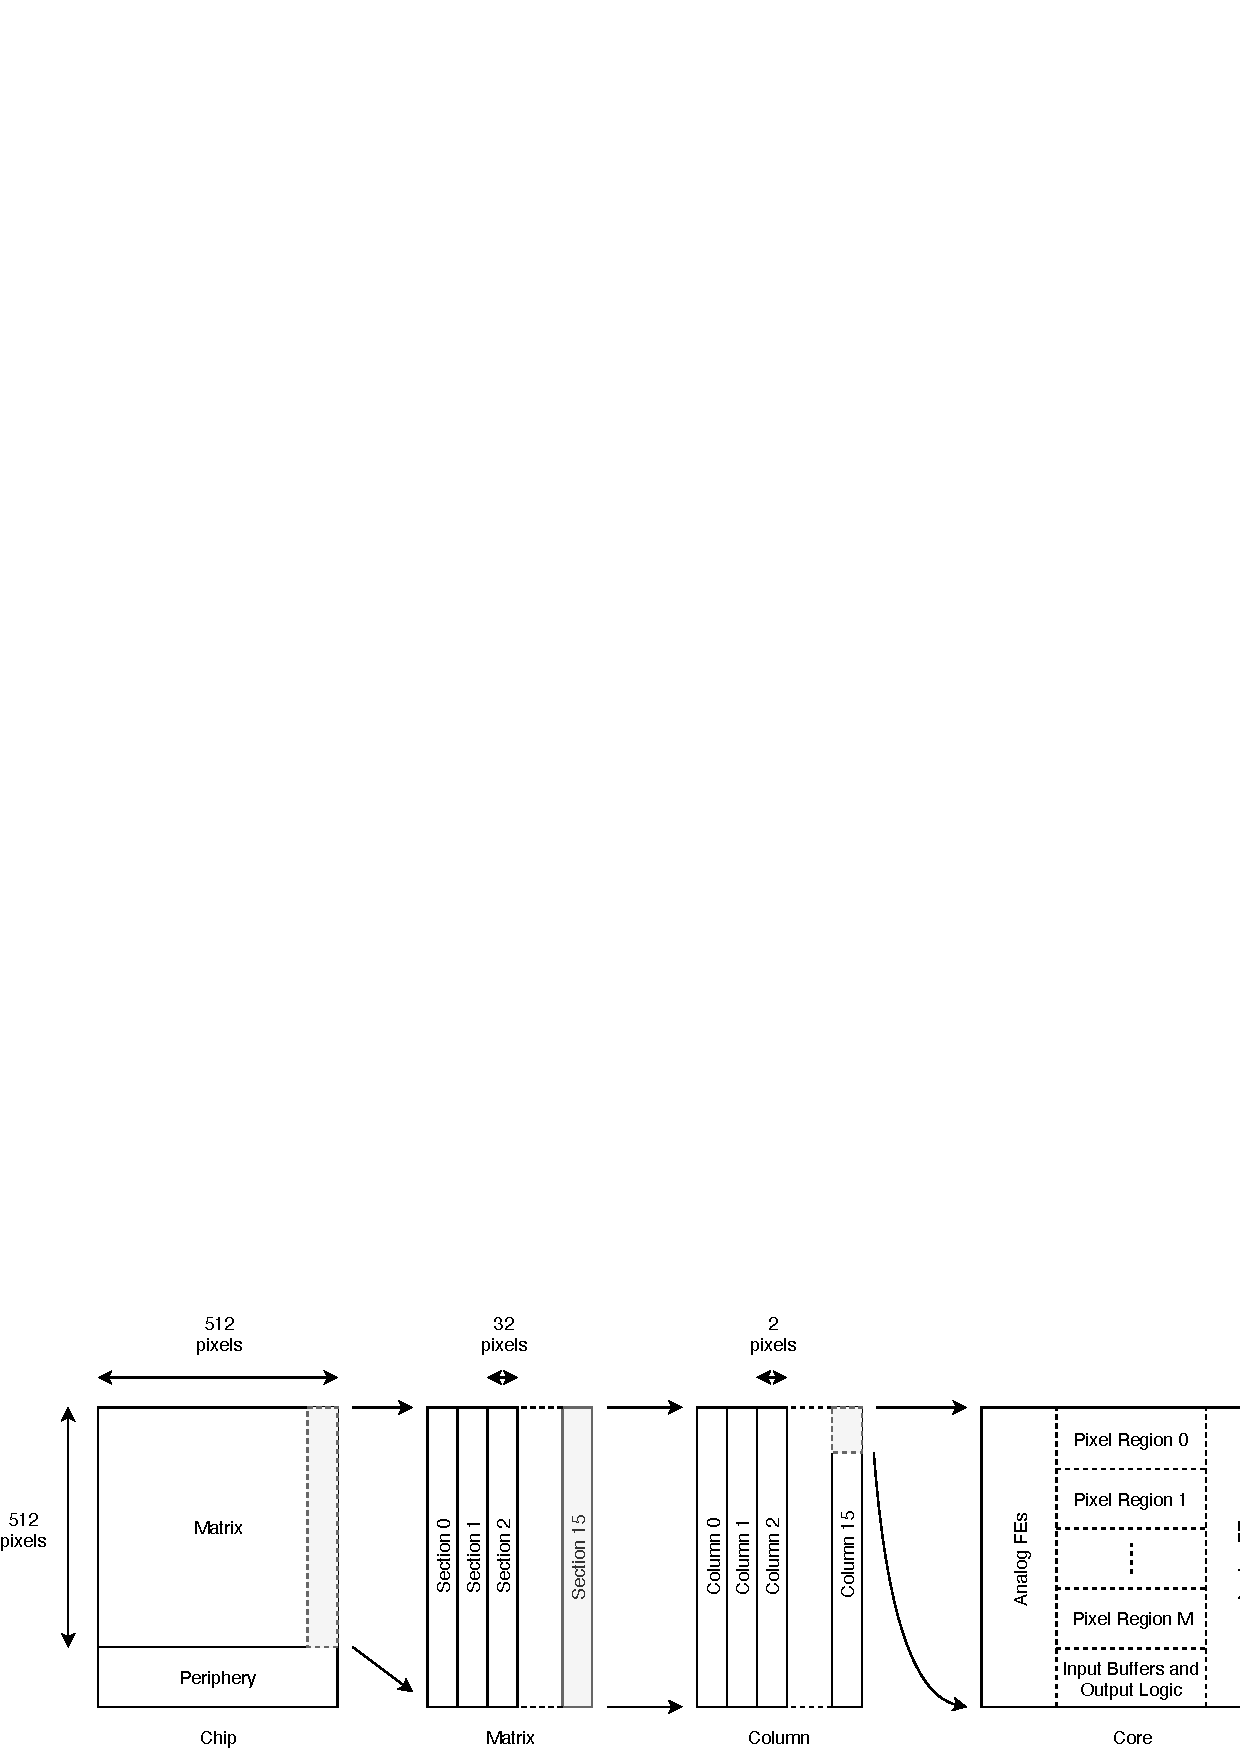
\includegraphics[width=.95\linewidth]{figures/ARCADIA/hierarchy.pdf}
            \caption{}
            \label{fig:hierarchy}
        \end{figure}

        
        \begin{figure}[h!]
            \centering
            \includegraphics[width=.95\linewidth]{figures/ARCADIA/token_chain.png}
            \caption{}
            \label{fig:token_chain}
        \end{figure}


        \begin{figure}[h!]
            \centering
            \includegraphics[width=.95\linewidth]{figures/ARCADIA/hadrhidr.png}
            \caption{}
            \label{fig:hadrhidr}
        \end{figure}
        


        \begin{figure}[h!]
            \centering
            \includegraphics[width=.95\linewidth]{figures/ARCADIA/clustering.png}
            \caption{}
            \label{fig:clustering}
        \end{figure}

        \begin{figure}[h!]
            \centering
            \includegraphics[width=.95\linewidth]{figures/ARCADIA/clustering_logic.pdf}
            \caption{}
            \label{fig:clustering_logic}
        \end{figure}
        


        Questa divisione si rispecchia in come sono fatti i dati: scrivi da quanti bit un
        dato è fatto e le varie cordinate che ci si trovano dentro; devi dire che c'è un pixel hot
        e spieghi dopo a cosa serve, e devi accennare al timestamp

        "A core is simply the smallest stepped and repeated instance of digital circuitry.
        A relatively large core allows one to take full advantage of digital sybthesis tools
        to implement complex functionality in the pixel matrix, sharing resources among
        many pixels as needed.".
        pagina 28 della review.\\



        TABELLA: con la gerarchia del chip
        Matrix (512x512 pixels)
        Section (512x32 pixels)
        Column (512x2)
        Core (32x2)
        Region (4x2)

        Nel chip trovi diverse padframe: cosa c'è nelle padframe e End of section.

        "DC-balance avoids low frequencies by guaranteeing at least one transition every
        n bits; for example 8b10b encoding n =5"



\chapter{Threshold and noise characterization}

\section{TJ-Monopix1 characterization}
    \subsection{Threshold and noise: figure of merit for pixel detectors}
        %python3 -i calibration/scurve_tot_histo.py -f calibration/calibration_data/20220506 -i 1 100 questo script crea i file di output contenenti i gli istogrammi del tot e della s curve
        %python3 -i calibration/tot_charge_plotting.py -f calibration/calibration_data/20220506 per fare il plot della s curve e relativi residui 
        %python3 -i calibration/tot_histo2d.py -f calibration/calibration_data/PMOS/20220506 per fare l'istogramma 2d del tot
        \red{Una caratterizzazione di soglia e rumore è necessaria in quanto questi valori condizionano sia le condizioni di operatività di questi chip, che le performance. }
        Infact, the signal to threshold ratio may be considered as the figure of merit for pixel detectors rather than the signal to noise ratio.
        The threshold has to be low enough to mantain a high signal efficiency, but also high enough to cut the noise: for a low threshold many pixels can fire at the same time and a positive feedback can set off a chain reaction eventually, causing all the other pixels to fire. 
        \red{Thus, the noise sets a lower bound to the threshold: if an occupancy $\leqslant$ $10^{-4}$ is required, for example, this correspond to the Gaussian 1-sided tail fraction for \SI{3.7}{\sigma}.
        In this case, if the noise is \SI{100}{e-}, for example, the threshold must be higher than \SI[parse-numbers=false]{3.7\times100}{e-}.}
        Typically this argument sets only a minimal bound to the threshold since the variation with time and from pixel to pixel have to be taken into account: the temperature, the anealing (for example, the radiation damages in the oxide layer causes shift of MOSFET threshold voltage) and the process parameters variation across the wafer (as for example process mismatch between transistors). 
        A requirement for the FE noise (the ENC is the equivalent input charge noise) is: 
        \begin{equation}
            ENC < \sqrt{(T/3.7)^2 - T_{RMS} ^2 (x) - T_{RMS} ^2 (t)}
        \end{equation}
        where the T is the threshold set, $T_{RMS}$ is the threshold variation during time (t) and across the matrix (x).

        For this reason is desiderable the possibility of changing and adapting the setting parameters of the FE, both in time and in space: this parameters are usually set by Digital to Analog Converter (DAC) with a number of bit in a typical range of 3-7.

        DAC elements require a lot of space that may be not enough on the pixel area. Therefore, the FE parameters are typically global, which means that they are assigned for the whole chip, or they can be assigned for regions the matrix is divided into. 
        The former case corresponds to TJ-Monopix1's design in which 7 bits are used for a total 127-DAC possible values, while the latter corresponds to the ARCADIA-MD1's one, \red{where quanti bit??}. 
        An other possibility, for example implemented in TJ-Monopix2, is allocate the space on each pixel for a subset of bits, then combinig the global threshold with a fine tuning. 

        To measure the threshold and noise of pixels a possible way is a scan with different known injected charge at a fixed threshold, that corresponds to the value where the efficiency of the signal exceeds the 50\%.
        Therefore, for a fixed threshold (I set IDB = 40 DAC to perform the scan) I have used the injection circuit available on the chip to inject 100 pulses for each input charge. 
        The injection comes on a capacity at the input of the FE circuit, whose mean value is \SI{230}{aF} (in section \ref{sec:} I'll present the calibration of the signal from which I also found the value of this capacity across the matrix). 
        For the PMOS flavors: since the DAC are biased at \SI{1.8}{V}, the Least significant Bit (LSB) corresponds to a voltage of \SI{14.7}{mV} from which the charge for LSB \SI{1.43}{e-/mV} and the conversion factor from DAC to electrons \SI{20.3}{e-/DAC} are obtained. 
        While this value is equivalent for all the PMOS flavor, the HV flavor is expected to have a different conversion factor, $\sim$ \SI{33}{e-/DAC}, beacuse of the different input capacity. 
    
        Besides the charge, also the duration and the period of the injection pulse can be set; it is important to make the duration short enough to have the falling edge during thed dead time of the pixel (in particular during the FREEZE signal) in order to avoid the afterpulse, coming at high input charge, triggering the readout and reading spurious hits. 
        \red{Questo problema è legato solamente all'impulso di iniezione di carica e non si ha invece con acquisizioni con sorgenti, come abbiamo verificato, e anche perchè. Immagine afterpulse oscilloscopio?}

        Assuming a gaussian noise, it can be described through the error function; actually, since the error function has y bounded between -1 and +1, the function I need is a modification of the $erf$: 
        
        \begin{equation}
            f(x, \mu, \sigma) = \frac{1}{2} \; \left(1\,+\,erf\left(\frac{x-\mu}{\sigma \sqrt{2}}\right)\right)
        \end{equation}
        \begin{equation}
            erf(z) = \frac{2}{\sqrt{\pi}} e^{-x^2} dx 
        \end{equation}   
            
    
        \begin{figure}[h!]
            \centering
            \includegraphics[width=.6\linewidth]{figures/charaterization/scurve.png}
            \caption{S curve for pixel (10, 10) of the PMOS flavor. The conversion of charge injected from DAC to electrons has been done assuming a conversion factor of \SI{20}{e-/DAC}.}
            \label{fig:scurve}
        \end{figure}   

        The mean minimum stable threshold modified through different generation of chips: in the 1st generation it was around \SI{2500}{e-} while in the 3rd (corresponding to nowadays chips) is less than \SI{500}{e-}. This allows in thinner sensors with smaller expected: from \SI{16000}{e-} produced in \SI{200}{\um}, down to \SI{2000}{e-} produced in \SI{25}{\um}. According with this \red{??}, the threshold of TJ-Monopix1 is around \SI{500}{e-}.
        \red{I successivi prototipi hanno una soglia e un rumore più bassi, ad esempio TJ-Monopix2 ha una soglia e un rumore... }
        
        
        La dispersione della soglia dopo al tuning e dovuta al dac è: 
        \begin{equation}
            \sigma_{THR, tuned} = \frac{\sigma_{THR}}{2^{n bit}}
        \end{equation}



        \begin{figure}[h!]
                -\begin{subfigure}{.5\textwidth}
                \centering
                \includegraphics[width=.99\linewidth]{figures/charaterization/threshold_histogram.png}
                \caption{}
                \label{fig:}
                \end{subfigure}
                \begin{subfigure}{.5\textwidth}
                \centering
                \includegraphics[width=.99\linewidth]{figures/charaterization/noise_histogram.png}
                \caption{}
                \label{fig:}
                \end{subfigure}
        \end{figure}            
           
        \begin{figure}[h!]
            \begin{subfigure}{.5\textwidth}
            \centering
            \includegraphics[width=.99\linewidth]{figures/charaterization/threshold_map.pdf}
            \label{fig:}
            \end{subfigure}
            \begin{subfigure}{.5\textwidth}
            \centering
            \includegraphics[width=.99\linewidth]{figures/charaterization/noise_map.pdf}
            \label{fig:}
            \end{subfigure}
            \caption{}
        \end{figure} 
    
    
        \begin{table}
                \begin{center}
                \begin{tabular}{| c | c | c |}
                \hline
                 & DAC units & electrons \\
                \hline
                \hline
                Threshold        & 24.529 $\pm$ 0.049 & \\
                                 &u: 24.433 $\pm$ 0.049 & \\ 
                                 &d: 24.623 $\pm$ 0.051 &    \\      
                Threshold dispersion & 1.848 $\pm$ 0.033 &\\
                                 &u: 1.867 $\pm$ 0.034 & \\ 
                                 &d: 1.825 $\pm$ 0.035 &    \\ 
                Noise            & 0.8222 $\pm$ 0.0043 & \\
                                 &u: 0.8225 $\pm$ 0.0045 & \\ 
                                 &d: 0.8221 $\pm$ 0.0043 &    \\      
                Noise dispersion & 0.0975 $\pm$ 0.0030 &\\
                                 &u: 0.0968 $\pm$ 0.0031 & \\ 
                                 &d: 0.0970 $\pm$ 0.0030 &    \\ 
                \hline
                \end{tabular}
                \caption{Flavor PMOS}
                \label{tab:}
                \end{center}
        \end{table}        
            
    
    I also have perfmorm a scan for different IDB value to verified the trend of the threshol.
                   
        

    \subsection{Calibration of the ToT}    
        %python3 -i acquisition_Fe55/fit_tot_single_pixel.py -f acquisition_Fe55/source_PMOSS/ per fare il fit    
        %python3 -i acquisition_Fe55/plot_tot_single_pixel.py -f acquisition_Fe55/source_PMOSS/ -fl 'gauss_line' per fare il plot di single pixel

        \begin{figure}[h!]
            \begin{subfigure}{.5\textwidth}
            \centering
            \includegraphics[width=.98\linewidth]{figures/charaterization/ToT_rollover.png}
            \caption{ToT rollover for pixel (10,10). The ToT is in range 0-64 since it is represented by 6 bit.}
            \label{fig:}
            \end{subfigure}
            \begin{subfigure}{.5\textwidth}
            \centering
            \includegraphics[width=.98\linewidth]{figures/charaterization/ToT_injection.png}
            \caption{}
            \label{fig:}
            \end{subfigure}
        \end{figure}    

        \begin{figure}[h!]
            \begin{subfigure}{.5\textwidth}
            \centering
            \includegraphics[width=.98\linewidth]{figures/charaterization/slope_histogram.png}
            \caption{}
            \label{fig:}
            \end{subfigure}
            \begin{subfigure}{.5\textwidth}
            \centering
            \includegraphics[width=.98\linewidth]{figures/charaterization/intercept_histogram.png}
            \caption{}
            \label{fig:}
            \end{subfigure}
        \end{figure} 

        \begin{figure}[h!]
            \begin{subfigure}{.5\textwidth}
            \centering
            \includegraphics[width=.99\linewidth]{figures/charaterization/slope_map.pdf}
            \label{fig:}
            \end{subfigure}
            \begin{subfigure}{.5\textwidth}
            \centering
            \includegraphics[width=.99\linewidth]{figures/charaterization/offset_map.pdf}
            \label{fig:}
            \end{subfigure}
            \caption{}
        \end{figure} 

        \begin{table}
            \begin{center}
            \begin{tabular}{| c |  c | c | c |c |}
            \hline
             & PMOS & & HV \\
            \hline
            \hline
            Slope [au/DAC] & 0.57145 $\pm$ 0.00025 \\
            Slope dispersion [au/DAC] &  0.01685 $\pm$ 0.00016\\
            Intercept [au] & -10.824 $\pm$ 0.019 \\
            Intercept dispersion [au] & 1.225 $\pm$ 0.013\\
            \hline
            \end{tabular}
            \caption{}
            \label{tab:}
            \end{center}
        \end{table}        

        \subsubsection{Absolute calibration}
        %python3 -i acquisition_Fe55/fit_tot_single_pixel.py -f acquisition_Fe55/source_PMOSS/Fe_acquisitions_6V/ per fare i fit. Attenzione che prende i file degli istogrammi npz già
        \begin{equation}
            f(x, m, q, N, \mu, \sigma) = m\,x + q + \frac{N}{\sigma \sqrt{2\pi}} e^{-\frac{1}{2}(\frac{(x-\mu)}{\sigma})^2}
        \end{equation}   
         
        \begin{figure}[h!]
            \begin{subfigure}{.5\textwidth}
            \centering
            \includegraphics[width=.99\linewidth]{figures/charaterization/fit_gauss_r69.pdf}
            \label{fig:}
            \end{subfigure}
            \begin{subfigure}{.5\textwidth}
            \centering
            \includegraphics[width=.99\linewidth]{figures/charaterization/fit_line_gauss_r69.pdf}
            \label{fig:}
            \end{subfigure}
            \caption{due pixel per far vedere la differenza tra i fit}
        \end{figure}            

        \begin{figure}[h!]
            \begin{subfigure}{.5\textwidth}
            \centering
            \includegraphics[width=.99\linewidth]{figures/charaterization/fit_gauss_r185.pdf}
            \label{fig:}
            \end{subfigure}
            \begin{subfigure}{.5\textwidth}
            \centering
            \includegraphics[width=.99\linewidth]{figures/charaterization/fit_line_gauss_r185.pdf}
            \label{fig:}
            \end{subfigure}
            \caption{due pixel per far vedere la differenza tra i fit}
        \end{figure}    

 
        
         \subsection{Fe vs bias}
         \begin{itemize}
             \item rate vs bias 
             \item posizione del picco del ferro vs bias    
             \item eventi sotto il picco vs eventi nella coda
         \end{itemize}
     
     
     \subsection{Measurements with radioactive sources}
         \red{CI metterei i plot con ferro, stronzio e cosmici}
         %python3 -i acquisition_Fe55/find_cluster.py -d acquisition_Fe55/source_PMOSS/noise_acquisitions_6V -> per cluster dimension e spettro del noise
         %python3 -i acquisition_Fe55/hit_map.py -f acquisition_Fe55/source_PMOSS/2022-04-07/2022-04-07_10-10-01_acq.h5 -> per le hit map, comprese qualche hitmap dei cluster
         %python3 -i acquisition_Fe55/Sr90_spectrum.py -d acquisition_Fe55/source_PMOSS/noise_acquisitions_6V/ -> per fare i plot dello stronzio
         ToT con doppia scala (calibrata in elettroni e non in ToT)
         hit per cluster
         dimensione cluster
         hit map di un paio di tracce?
        \subsection{Dead time measurements}
        The hit loss is due to analog and digital pile up: the first one occurs when a new hit arrives during the pre-amplifier response, the second instead, which is the more relevant contribution with high rate, while the information of the previous hit has not yet been transferred to the periphery.  
        As only one hit at a time can be stored on the pixel's RAM, until the data have completed the path to get out, the pixel is paralyzed and the dead time $\tau$ almost corresponds with the time needed to trasmit the data-packets off-chip.
        Since the exportation of data from pixel to the EoC occurs via a 21-bits data bus, only one clock cycle is need to transfer the data to the end of column and the dead time bottleneck is given by the bandwidth of the serializer at the EoC. In our setup the serializer operates at 40 MHz, thus to transmit a data packet (27-bit considering the addition at the EoC) at least \SI{675}{ns} are needed. 
        For what we have said so far, the R/O is completely sequential and therefore is expected a linear dependence of the reading time on the number of pixels to read:
        \begin{equation}
            \tau =\, 25\: \unit{ns}\, \times\, (\alpha\, N +\, \beta)
            \label{eq:reading_time}
        \end{equation}
        where $\alpha$ and $\beta$ are parameters dependent on the readout chain setting. 
        
        To measure and test the linearity of the reading time with the number of pixels firing, I have used the injection mode available on the chip. 
        Indeed, the injection mode allows fixing not only the amplitude of the pulse, which corresponds to the charge in DAC units, but also the period and the width.
        I have injected a fix number of pulses (100) and looked for the rate when the efficiency decreases. 
        Moreover to test that there is no dependece of the digital readout time from the charge of the pulse, I have try to change the amplitude of the pulse injected, but the parameters found were consistent with the default configuration ones.

        \red{Al posto degli esempi con 5 e 10 pixels metterei un esempio dell'efficienza vs il periodo quando leggo un singolo pixel. Una cosa che volevo fare era anche provare a fittare la slope con cui l'efficienza scende: se la slope è uguale per tutti il readout diventa completamente predittivo. }
        \begin{figure}[h!]
            \begin{subfigure}{.5\textwidth}
            \centering
            \includegraphics[width=.98\linewidth]{figures/charaterization/efficiency_5pixels.png}
            \caption{\red{efficiency vs DELAY 5 pixels}}
            \label{fig:}
            \end{subfigure}
            \begin{subfigure}{.5\textwidth}
            \centering
            \includegraphics[width=.98\linewidth]{figures/charaterization/efficiency_10pixels.png}
            \caption{\red{efficiency vs DELAY per 10pixels}}
            \label{fig:}
            \end{subfigure}
        \end{figure}
        
        While the single pixel reading time and the dead time do not depend on the position on the pixel matrix and are equal to \red{106 (46+60)} clock counts within 1 clock count, on the other hand the $\tau$ depends on the pixel position on the matrix when more than one pixel are firing. 
        In particular the priority chain goes from row 224 to row 0, and from col 0 to 112, that means the last pixels to be read is the one on le bottom right corner of the matrix. 

        In figure \ref{fig:dead_time} is reported the reading time versus the number of pixels injected; the R/O parameters that control the reading time and their default values are reported on table \ref{tab:tab:R/O_param}.
        \begin{table}
            \begin{center}
            \begin{tabular}{|c | c | c |}
            \hline
            Parameter & Value [\si{DAC}] & Value [\si{\us}]\\
            \hline
            \hline
            START\_FREEZE & 64 & 1.6\\
            STOP\_FREEZE & 100 & 2.5\\
            START\_READ & 66 & 1.65\\
            STOP\_READ & 68 & 1.7\\
            \hline
            \end{tabular}
            \caption{Default configuation of the R/O parameters}
            \label{tab:R/O_param}
            \end{center}
        \end{table}

        The factor $\alpha$, referring to eq. \ref{eq:reading_time} is proportional to the difference (STOP\_FREEZE - START\_READ), while the offset $\beta$ lies between 5 and 15 clock counts.
        Since through the injection a random hit rate on the matrix can't be simulated, as the coordinates of the pixels to inject must be specified, for convenience I used the pixels on the same column/row. No difference in the $\alpha$ and $\beta$ coefficients has been observed between the two case. 
        \begin{figure}[h!]
            \centering
            \includegraphics[width=.9\linewidth]{figures/charaterization/default_line.png}
            \caption{}
            \label{fig:dead_time}
        \end{figure}

        \begin{figure}[h!]
            \centering
            \includegraphics[width=.9\linewidth]{figures/charaterization/parameters_points.png}
            \caption{}
            \label{fig:dead_time}
        \end{figure}        

        \red{Ci sarebbe da spiegare perchè i parametri che usiamo noi come default non sono quelli che minimizzano il tempo di lettura. La spiegazione è che "Abbiamo copiato i valori dal repositorio di quelli di Bonn". Un'altra domanda potrebbe essere: come mai non ho esplorato una zona più vasta per i parametri del R/O. Cambiando molto i parametri del R/O la lettura non funzionava per niente: ad esempio CONF\_STOP\_FREEZE non può essere impostato nè sopra 105 nè sotto 95}



\section{ARCADIA-MD1 characterization}


\appendix
\chapter{Pixels detector: a brief overview}
\section{Signal formation}
    When a charge particle passes through a pixel and loses energy by ionization a part of that energy is used to generate electron-hole pairs (an other part is used for other processes, as the lattice excitation) which are then separated by the elettric field and collected at their respectivelly electrodes ($p$ for holes and $n$ for electrons)\footnote{Even if in principle both the electrode can be used to read a signal, for pixel detectors, where the number of channel and the complexity of readout are high, only one is actually used. In strip and pad detectors, instead, is more common a dual-side readout}; by the drift of these charges, a signal $i_e$ is generated on the  electrode $e$ as stated by the Shockley–Ramo's theorem: 
    \begin{equation}
        i_e(t) = -q\: v(t)\, E_{WF,e}
    \end{equation}
    where $v(t)$ is the instantaneous velocity of the charge $q$ and $E_{WF}$ is the weighting field, that is the field obtained biasing the electrode $e$ with 1V and all the others with 0V.\\
    The drift velocity of the charge depends on the elettric field and on the mobility of the particle:
    \begin{equation}
        v = \mu(E)\, E
    \end{equation}
    where $\mu(E)$ is a function of the electric field and is linear with $E$ only for small $E$: at highter values the probability of interactions with optical phonons increases and the mobility drops and this leads to an indipendency of the velocity from the electric field (fig. \ref{fig:mobility_drift2}).\\
    SECONDO ME MANCA ANCORA UNA FRASE DI CONNESSIONE\\
    \begin{figure}[h!]
        \begin{subfigure}{.5\textwidth}
        \centering
        \includegraphics[width=.8\linewidth]{figures/Pixel_detectors/mobility_in_semiconductor.png}
        \caption{Typical values for elecrons and holes mobility 
        in silicon at room temperature are $\mu _n \sim$ 1450 $cm^2/Vs$, $\mu _h = 500$}
        \label{fig:mobility_drift1}
        \end{subfigure}
        \begin{subfigure}{.5\textwidth}
        \centering
        \includegraphics[width=.8\linewidth]{figures/Pixel_detectors/velocity_in_semiconductor.png}
        \caption{Drift velocity at room temperature in different semiconductors}
        \label{fig:mobility_drift2}
        \end{subfigure}
        \label{fig:mobility_drift}
    \end{figure}

    The average energy needed to create a pair at 300 K in silicon is $w_i$ = 3.65 eV, that is more than the mean ionization energy because of the interactions with phonon, hence for a MIP the most probable value of charge released in the semiconductor (assuming a stopping power in silicum of 1 MeV g/$cm^2$) is: 
    \begin{equation}
        \langle \frac{dE}{dx}\rangle \frac{1}{w_i} \sim 100 \: e/h \sim \frac{1.6 \:10^{-2}fC}{\mu m}
    \end{equation}
    It is foundamental that pairs e/h are produced in the depleted region of the semiconductor where the probability of recombination with charge carriers is low to avoid loss of signals.\\
    Pixel detectors are then commonly reverse biased: a positive bias is given to the $n$ electrode and a negative to the $p$
    to grow the depletion zone in the epitaxial layer below the electrode. The width of the depletion region is related with the extern bias $V_{ext}$, the resistivity $\rho$ and also with the dopant:
    \begin{multicols}{2}
        \begin{equation}
            d_{n} \sim 0.55 \sqrt{\frac{\rho}{\Omega cm}\frac{V_{ext}}{V}} \mu m 
        \end{equation}\break
        \begin{equation}
            d_{p} \sim 0.32 \sqrt{\frac{\rho}{\Omega cm}\frac{V_{ext}}{V}} \mu m
        \end{equation}
        \label{eq:deplation_d}
    \end{multicols}
    DA DOVE VENIVA QUESTA DIFFERENZA? DALLA MOBILITÀ MA NON MI RICORDO COME CI SI ARRIVAVA.\\
    For that reason high resistivities wafer (100 $\Omega cm - k\Omega cm$) are typically prefered beacause they allow bigger deplation zone with smaller voltage bias. 

\section{Radiation dameges}
    Radiation hardeness is a fundamental requirement for pixels detector especially in HEP since they are almost always installed near the interaction point where there is a high energy level of radiation. At LHC the $\phi_{eq}$ per year in the innermost pixels detector is $10^{14} n_{eq}/cm^2$; this number reduces by an order passing to the outer tracker layer. (referenza: pag 341 Wermes)\\ 
    Here the high fluence of particles can cause a damage both in the substrate of the detector and in the superficial electronics. 
    
    The first one has a principal non ionising nature (non ionizing energy loss, NIEL) since it is related with the dislocation of the lattice caused by the collision with nuclei; by this fact the NIEL hypothesis states that the substrate damage is normalized to the damage caused by 1 MeV neutrons. Differently, surface damages are principally due to ionising energy loss.

    DUE PAROLE IN PIÙ SUL SURFACE DAMAGE\\
    a charge accumulation in oxide ($S_iO_2$) can cause the generation of parasitic current with an obvious increase of the 1/f noise.\\
    Anyway surface damages are less relevant then the previous one since with the development of microelectronics and with the miniaturization of components (in electronic industry 6-7 nm transistors are already used, while for MAPS the dimensions of components is around 180 nm) the quantity of oxide in circuit is reduced.

    Let's spend instead two more other words on the more-relevant substrate damages: the general result of high radiation level is the creation of new energy levels within the silicon band gap and depending on their energy-location their effect can be different, as described in the Shockely-Read-Hall (SRH) statistical model.
    \begin{figure}
        \begin{subfigure}{.5\textwidth}
        \centering
        \includegraphics[width=.8\linewidth]{figures/Pixel_detectors/type_inversion.png}
        \caption{1a}
        \label{fig:type_inversion}
        \end{subfigure}%
        \begin{subfigure}{.5\textwidth}
        \centering
        \includegraphics[width=.8\linewidth]{figures/Pixel_detectors/type_inversion.png}
        \caption{1b}
        \label{fig:type_inversion}
        \end{subfigure}
    \end{figure}
    The three main consequence of radiation damages are the changing of the effect doping concentration, the leakage current and the increasing of trapping probability.

    \textbf{Changing of the effective doping concentration:} is associated with the creation/removal of donors and acceptors center which trap respectively electrons/holes from the conduction band and cause a change in effective space charge density. Even an inversion (p-type becomes n-type\footnote{L'INVERSIONE OPPOSTA NON CE L'HAI PERCHÈ L'INVERSIONE È ASSOCIATA AD UN CAMBIO DELLA CONCETRAZIONE DA ... A ...\\E COME MAI L'ALTRO NON È FAVORITO?}) can happen: indeed it is quite common and happens at not too high fluences ($\phi_{eq} 10^{12-13}n_{eq}cm^{-2}$). 
    A changing in the doping concentration requires an adjust of the biasing of the sensor in time (eq.\ref{eq:deplation_d}) and sometimes can be difficult keeping to fully deplete the bulk.

    \textbf{Leakage current:} is associated with the generation-recombination centres. It has a strong dependence with the temperature ($I_{leak}\propto T^2$), whose solution is therefore to operate at lower temperature.

    \textbf{Increase of trapping probability:}  È ASSOCIATA CON QUALE TIPO DI CREAZIONE DI LIVELLO ENERGETICO?
    since the trapping probability is costant in the depleted region, the collected charge decreases exponentially with the drift path. The exponential coefficient, that is the mean trapping path, decreases after irradiation and typical values are 125-250 $\mu m$ and must be compared with the thickness of the depleted region which () corresponds to the mean drift path.

    Different choises for substate resistivity, for junctions type and for detector design are typically made to fight radiation issues. Some material with high oxygen concentration (as crystall produced using Czochralki (Cz) or float-zone (Fz) process (CONTROLLA SE SONO LORO QUELLI GIUSTI)) for example, show a compensation effect for radiation damage; an other example is the usage of n+ -in-p/n sensors (even if p+ -in-n sensors are easier and chieper to obtain) to get advantage of inversion/to have not the inversion (since they are already p-type). After inversion the n+p boudary, coming from n+ in-n, but to keep using the sensor the depletion zone still must be placed near the diode\footnote{With inversion some isolation process of electrodes can become important and p-spray/p-stop tecnique can eventually be applied. PERCHÈ CON L'INVERSIONE TI POTREBBE SERVIRE UNA TECNICA DI ISOLAMENTO?}.
    
    
    Radiation damage in CMOS circuits is entirely due to charge
    carriers generated by ionization in the dielectric layers of the
    process

\chapter{FLASH radiotherapy}
La radioterapia si usa nel 60 per cento dei pazienti, sia come cura che come trattamento palliativo. Si associa spesso ad altre cure e si può fare prima/durante/dopo un intervento.\\

Si può fare in modi diversi: da dentro (brachytherapy) oppure da fuori (quella standard). Un requisito importante è la delinazione del target (non vuoi rischiare di beccare i tessuti sani), per cui prima tipicamente si fanno esami di imaginig del tumore. TIpicamente anche gli acceleratori stessi per la terapia sono provvisti di radiografia.

Un problema dei fotoni ad esempio è che il loro rilascio di dose è lineare, per cui danneggi anche i tessuti sani. Il problema dei protoni invece è che hanno un picco troppo strtto per cui non puoi coprire grosse zone e sorpattuto se sbagli rischi davvero di danneggiare moooolto i tessuti sani.\\

\section{Cell survival curves}
Curva di efficacia del trattamento in funzione della dose:
\begin{equation}
    \frac{S(D)}{S(0)}=e^{-F(D)}
\end{equation} 
dove F(D)   
\begin{equation}
    F(D) = \alpha D + \beta D^2
\end{equation} 
dove $\alpha$ e $\beta$ rappresentano due tipi di danno diversi: coefficients, experimentally determined, characterizing the
radiation response of cells. In particularly, alpha represents the rate of cell killing
by single ionizing events, while beta indicates the maximal rate of cell killing by
double hits observed when the repair mechanisms do not activate during the
radiation exposure.
Si ottiene una curva di sopravvivenza dove si vede la possibilità delle cellule di autoripararsi. A basse dosi infatti le cellule possono ripararsi.\\

Per introdurre l'effetto FLASH instroduco prima la therapeutic window.  \\

TCP è la tumor control Probability che indica la probabilità delle cellule del tumore di essere uccise dopo una certa dose (con in riferimento a dose in acqua)\\
Se una media di $\mu(D)$ di cellule di tumore are killed con una dose D, la probabilità che n cellule sopravvivono è data da $P(n|\mu)$ poisson:
\begin{equation}
    P(n|\mu) = \frac{\mu(D)^ne^{-\mu(D)}}{n!}
\end{equation}    

\begin{equation}
    TPC(D) = P(n=0|\mu(D))= e^{-\mu(D)}
\end{equation} 
D'altra parte hai una probabilità di fare danno su normal tissue NTCP Normal Tissue Complication Probability, che rappresenta il problema principale e che limita la massima radiazione erogabile\\
Una scelta bilanciata si applica guardando a questi due fattori; si usa il therapeutic index definito come TCP/NTCP.\\
La cosa ottimale è ampliare la finestra del therapeutic ratio.\\


CONV-RT 0.01-5 Gy/min. A typical RT regime today consists of daily franctions of 1.5 to 3 Gy given over several weeks.\\
Nell Intra operative radiation therapy (IORT), where they reach values respectively about
20 and 100 times greater than those of conventional radiation therapy.

FLASH vuole ultrahigh mean dose-rate (maggione di 40 Gy/s) in modo da ridurere anche il trattamento a meno di un secondo. \\



\section{FLASH effect}
Ci sono due effetti che affect the flsh effect and la sua applicabilità: Dose rate effect e oxygen\\

Cellule che esibiscono hypoxia (cioè cellule che non hanno ossigeno sono radioresistenti); al contrario normoxia e physoxia non lo sono.
la presenza di ossigeno rende la curva steeper indicando che lo stesso danno si raggiunge a livelli di dose più bassi rispetto al caso senza ossigeno.\\
FIGURA con una curva a confronto con e senza ossigeno.\\
Typically, the OER is in the order of 2.5–3.5 for most cellular systems


Quindi si vogliono sfruttare questi effetti per diminuire la tossicità sui tessuti sani\\







\printbibliography[heading=bibintoc, title={Bibliography}] 
\end{document}



